\section{Evaluation}
\label{section:evaluation}

%\begin{enumerate}
%	\item Evaluierung interessanter Aspekte anhand von Statistiken
%\end{enumerate}

When performing fully automated fuzzing, the full fuzzing process for one message takes around 5.2 seconds. The majority of time is consumed by the processing of the message on the constrained device. \Autoref{figure:fuzzing_performance} displays the processing time of a CoAP message with a different number of header fields by the constrained devices.

This shows TODO

% This time can highly vary and depends heavily on the number given options in the CoAP message.
Setup times for the devices can vary due to cached binaries but can reach the magnitude of several minutes.

\begin{figure}[h]
	\centering
	TODO
	% 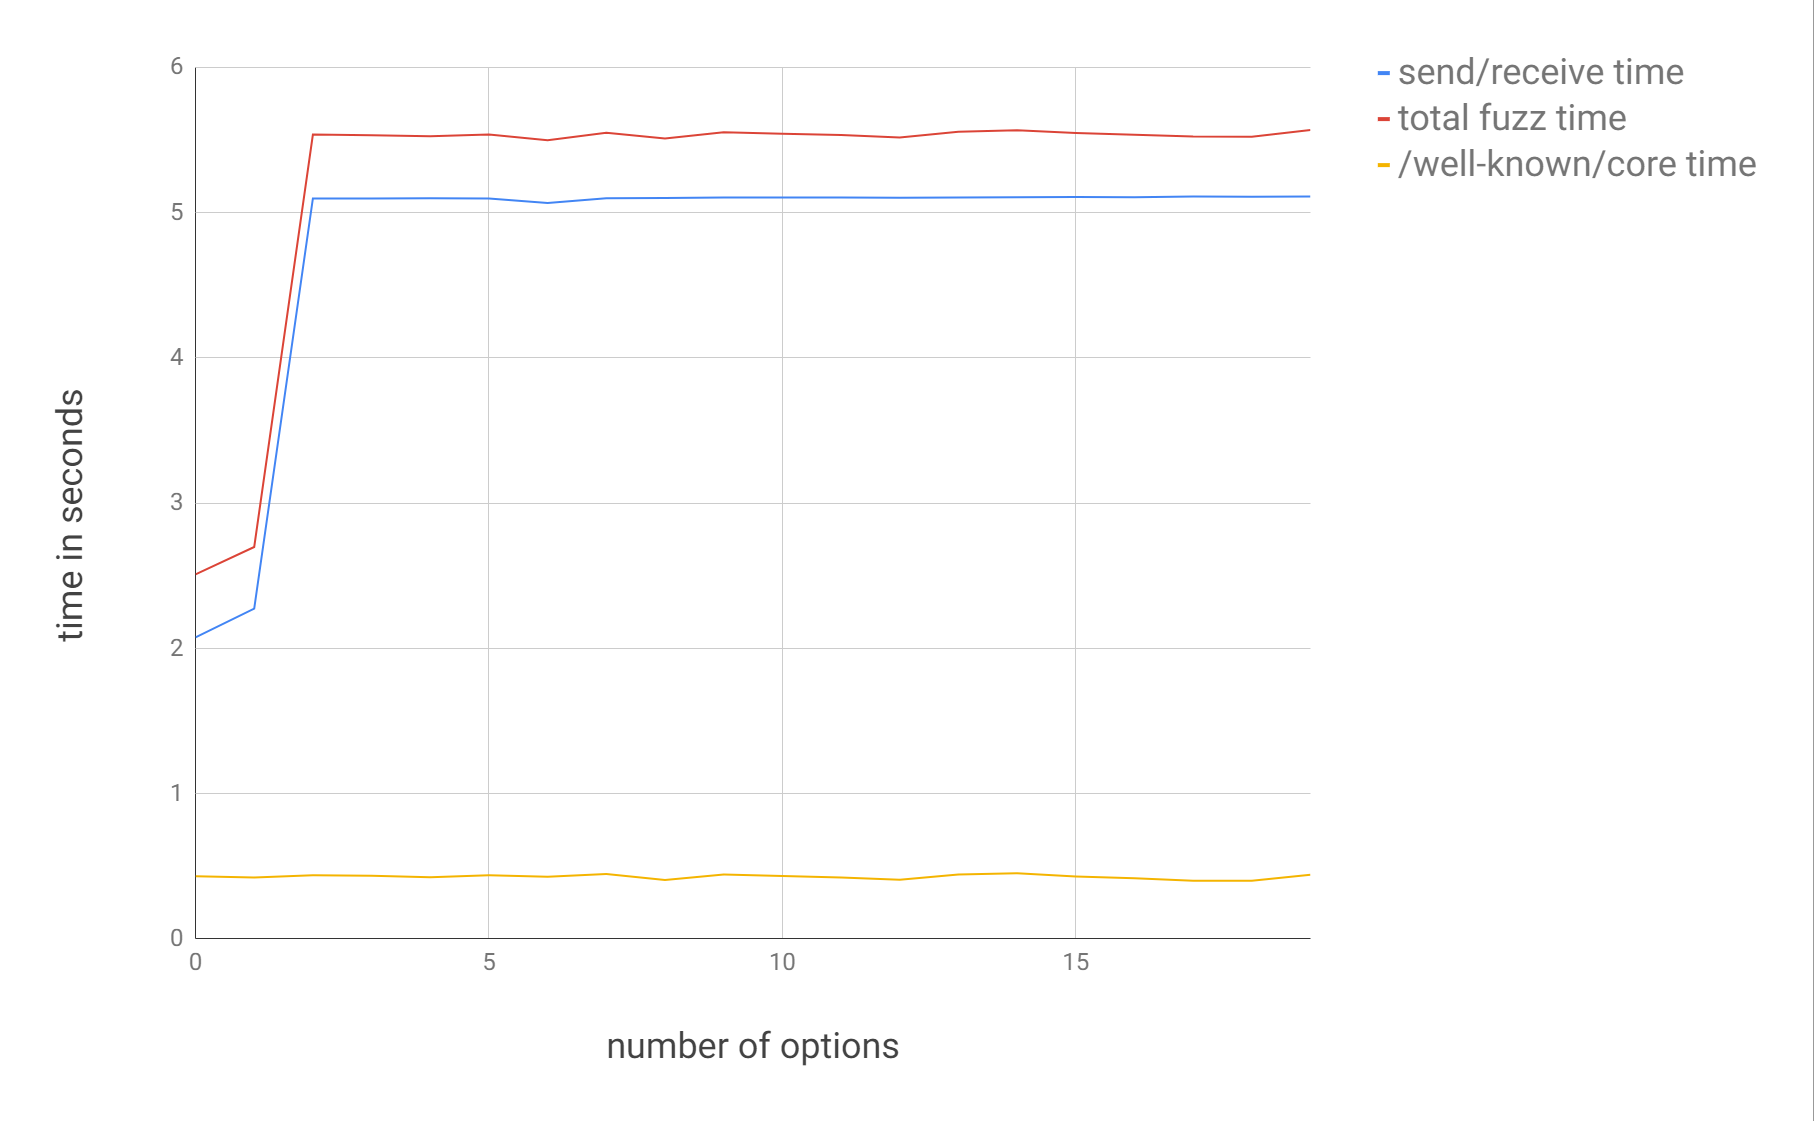
\includegraphics[width=0.5\textwidth]{images/fuzzing_performance}
	\caption{Processing time of CoAP messages with different amounts of options}
	\label{figure:fuzzing_performance}
\end{figure}[h]

In order to evaluate the fuzzer and the system under test, we performed 60.000 fuzzing requests but did not succeeded in causing a crash or a device malfunction. In order to make sure that potential crashes can be found by our setup, we temporarily added an infinite loop to the CoAP implementation of Contiki-NG. This loop was entered if the token length had a specific value and the hardware watchdog subsequently triggered a restart. All of these expected crashes were properly tracked by our fuzzer.